\documentclass[a4paper,12pt]{article}

\usepackage{utc-article}
\usepackage{lipsum} % for generating random text
\usepackage{multicol} % to have multiple colums in one document

\title{UTC \LaTeX : Article}
\author{John DOE}
\date{\today}

\uv{SY02}
\semester{A23}
\branche{GI}
\filiere{Apprentissage}

\setlength{\parindent}{0cm}

\begin{document}

\articletitle

\begin{multicols}{2}

\textbf{Part 1} \\
\lipsum[1][1]
\lipsum[1][2]
\lipsum[1][3]
\lipsum[1][4]
\lipsum[1][5] \\

\textbf{Part 2} \\
\lipsum[2][1]

\begin{figure}[H]
\centering
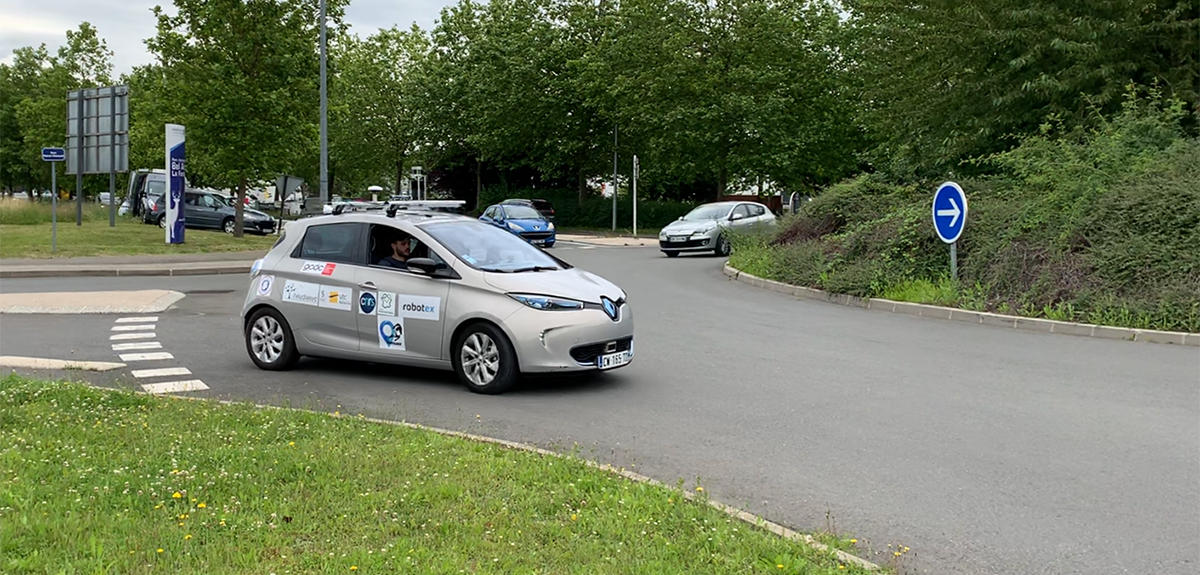
\includegraphics[width=\linewidth]{img/zoe_hds.jpg}
\caption{Illustration intégrée dans une seule colonne avec un float.}
\end{figure}

\lipsum[2][2]
\lipsum[2][3]
\lipsum[2][4]

\textbf{Part 3} \\
\lipsum[3]

\textbf{Conclusion} \\
\lipsum[4]

\end{multicols}

\end{document}
